\documentclass[11pt]{article}
\usepackage{amsmath,amsthm,verbatim,amssymb,amsfonts,amscd, graphicx}
\usepackage{graphicx}
\usepackage{subcaption}
\usepackage{listings}
\usepackage{float}
\usepackage{url}
\usepackage{titlesec}
\setcounter{secnumdepth}{4}


\graphicspath{{./times/}}
\topmargin0.0cm
\headheight0.0cm
\headsep0.0cm
\oddsidemargin0.0cm
\textheight23.0cm
\textwidth16.5cm
\footskip1.0cm

\titleformat{\paragraph}
{\normalfont\normalsize\bfseries}{\theparagraph}{1em}{}
\titlespacing*{\paragraph}
{0pt}{3.25ex plus 1ex minus .2ex}{1.5ex plus .2ex}


\begin{document}
\title{CS 5220\\ Project 3 - All Pairs Shortest Path}
\author{Marc Aurele Gilles (mtg79)\\ Edward Tremel (ejt64) \\ Yu Su (ys576)}
\maketitle

\section{Introduction}
In this project the goal is to profile, parallelize and tune an algorithm which computes the shortest path between all the pairs in a graph.


\section{Profiling of Original Code}
The profiling was done using amplxe. By looking at the hotspots report, we observe that most of the time (45 out of 67 seconds) is spent in the \texttt{square} function, which is to be expected as all of the computation is done in this function. A notable point, however, is that virtually all the rest of the time is spent waiting, which seems to indicate a significant load imbalance between the threads.
Looking at the time spent inside of the \texttt{square} function, we observe that a majority of the time (27 out of 45 seconds) is spent fetching memory and writing it to a float, which could indicate that there is poor cache utilization.

This profiling leads us to believe that we should try to address two problems for the OMP implementation: have better load balancing, and increase cache reuse.



\section{Initial MPI Implementation}
For our MPI implementation, we assign each processor to a large block of the matrix instead of an entire column as the original code does.
Note that to update one entry of the matrix for one step of the outer loop we need to read the whole column and row of that entry. 
Therefore, if each processor is assigned to a column, each processor needs to access each other column, and thus needs to communicate with all of the other processors. 
By assigning each processor to a block of the matrix instead, we allow each processor to have to communicate with only the blocks that share its row and its column.
We believe this will alleviate the load balancing problem seen in the OpenMP code.

To avoid global communications with this blocking strategy, we create $2n_{block}$ groups and communicators, where $n_{block}=n/blocksize$. 
Here $n$ is the dimension of the matrix and $blocksize$ is the dimension of the blocks. 
That is, we have one communicator for each row of blocks, and one communicator for each column of blocks. 
Each thread, which owns its own block, is then added to the communicator of its row and to the communicator of its column. 
Therefore each thread is in two different communicators (in addition to the world communicator), but no two threads are in the same two communicators.
To update its block, each processor makes one \textbf{\texttt{MPI\_Allgather}} call in its column communicator and one \textbf{ \texttt{MPI\_Allgather}} call in its row communicator, which reads all of the entries in its block column and block row, performs the update on its own block, and calls \textbf{\texttt{MPI\_Allgather}} again to share its result with the other processors.

The number of entries to be shared in this manner is $2 \cdot n \cdot blocksize$ per thread and per time step, compared to $n^2$ if each thread owned a column instead.

\section{Performance of Initial MPI Implementation}
We measured the runtime of our MPI implementation for various numbers of processors and compared it to the original OpenMP code running with various numbers of processors.
Unfortunately, since our MPI implementation cannot handle non-square numbers of processors, we were only able to test it with 1, 4, and 16 processors (a maximum of 24 processors are available on the Xeon main boards).
Figure \ref{fig:mpi-omp} shows the results for numbers of processors greater than 1.
The serial versions of both programs were so slow that we plotted them on a separate graph, figure \ref{fig:serial}.

\begin{figure}[h]
	\centering
	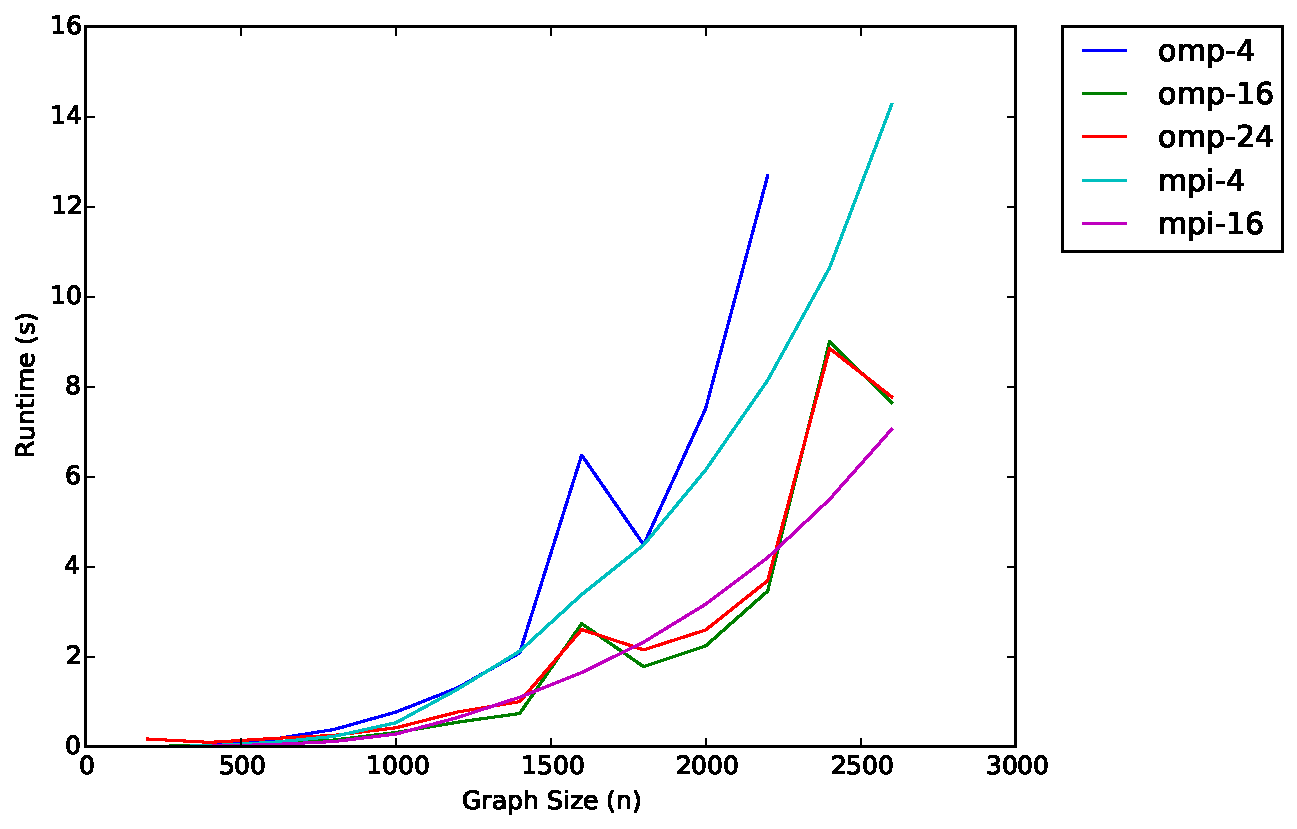
\includegraphics[width=.7\textwidth]{mpi_omp_comparison.pdf}
	\caption{Speed of the OpenMP and MPI implementations as the problem size and number of processors changes.}
	\label{fig:mpi-omp}
\end{figure}

\begin{figure}[h]
	\centering
	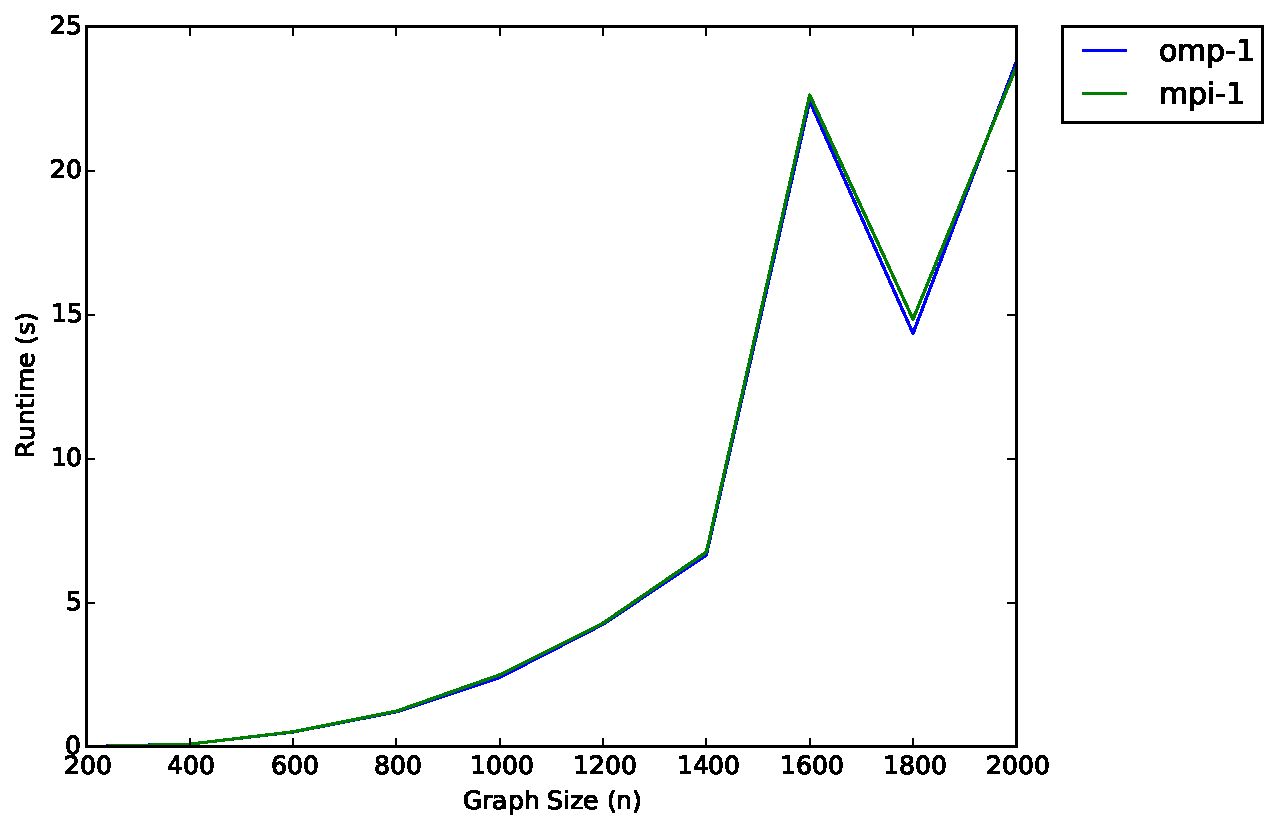
\includegraphics[width=.6\textwidth]{serial.pdf}
	\caption{Speed of the OpenMP and MPI implementations with only one processor.}
	\label{fig:serial}
\end{figure}

With a small number of processors (4), our MPI implementation runs about as well as the OpenMP code for small values of $n$, and scales much better for large values of $n$.
With 16 processors, our MPI implementation is actually a little slower than the OpenMP code at small values, and for some reason much slower for values of $n$ between 1800 and 2200.
However, for $n = 1600$ and also for large values of $n$, we again perform faster than OpenMP.


\section{Tuning the MPI Implementation}
After profiling the MPI implementation, we observed that most of the time was spent doing memory accesses. Therefore, we tried to optimize our MPI implementation by increasing the cache hits. 
Similarly to how we tuned matrix multiplication, we used kernel which uses a blocking strategy (on top of the blocking which is used for the parallelization), and copy optimization. 
Furthermore, we used aligned memory allocations to ease vectorization. 


We can increase cache utilization by subdividing each block into smaller blocks chosen to fill a thread's local cache.
The idea is similar to the matrix multiplication problem since they have a similar formulation.
With the Xeon E5-2620 v3, each core has 256KB L2 cache, so we choose a block size of 128. 
We apply copy optimization by using \texttt{\_\_mm\_\_malloc} to allocate buffers with a byte alignment of 64 bits. 
The reason that this byte alignment gives the best performance may be because the size of an integer in a 64-bit core is 64 bits. 

We tested our optimized block square function in a single thread and found that it runs in 80s with n=3072, compared with 350s spent in the original square function in a single thread. 
Thus the second level of blocking improves performance significantly even without parallelization. 
However, directly applying \texttt{\#pragma parallel for} to the sub-blocked version fails, so we only applied the optimized kernel to the MPI version.

\section{Performance Analysis of Tuned MPI}
To get an idea of how much our optimized kernal improved the MPI implementation, we tested its runtime on various graph sizes and compared it to our original MPI implementation and the OpenMP implementation.
We ran all three implementations with 16 threads, the largest number our MPI implementation can support due to its assumption that the number of threads is square.
Figure \ref{fig:size-comparison} shows that the optimized kernel gives us modest improvements at small problem sizes, but significant improvements at large problem sizes, especially over the OpenMP implementation which seems to suffer a catastrophic breakdown at problem sizes over n=4000.

\begin{figure*}[ht]
	\centering
	\begin{subfigure}[b]{.45\textwidth}
		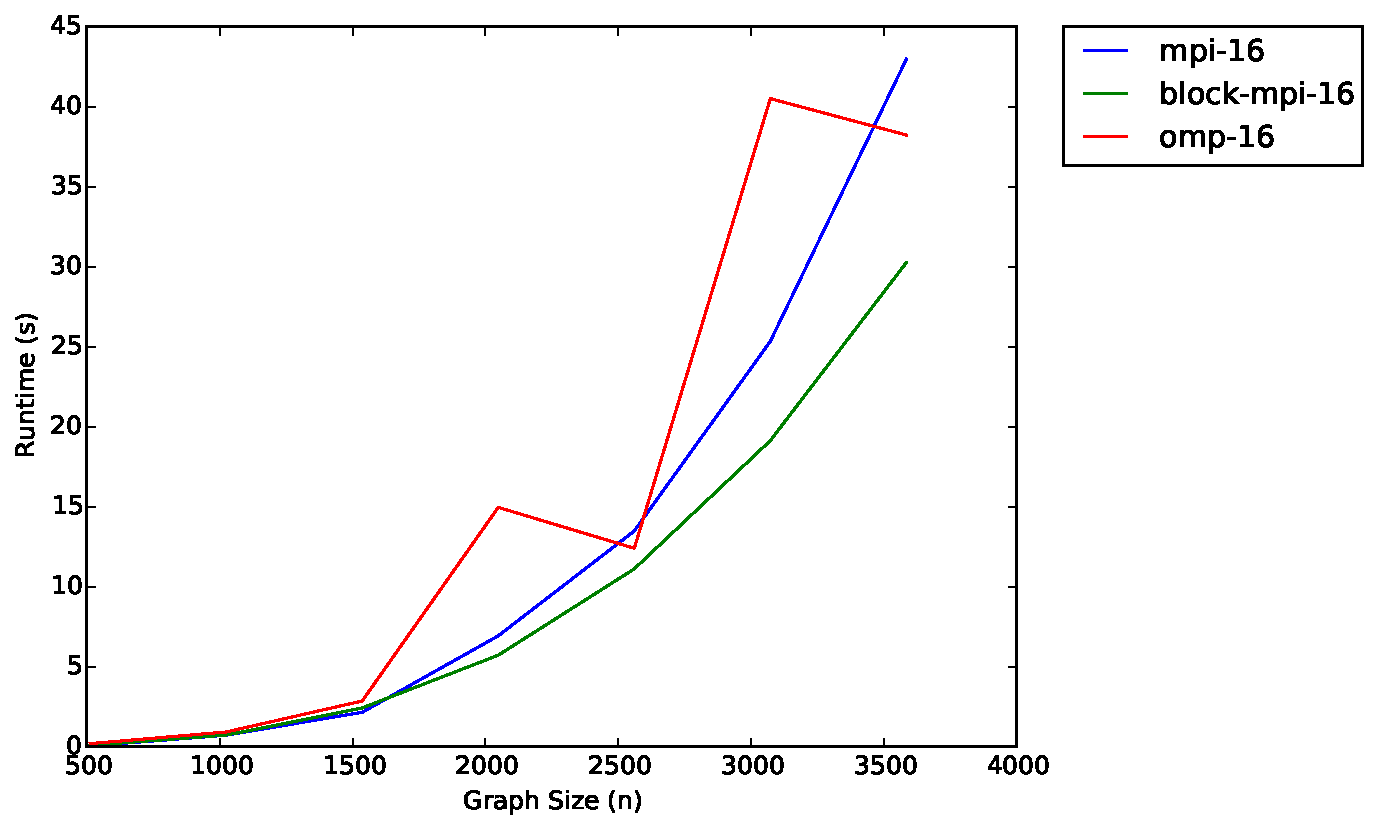
\includegraphics[width=\textwidth]{comparison_small.pdf}
		\caption{Small problem sizes}
	\end{subfigure}
	\begin{subfigure}[b]{.45\textwidth}
		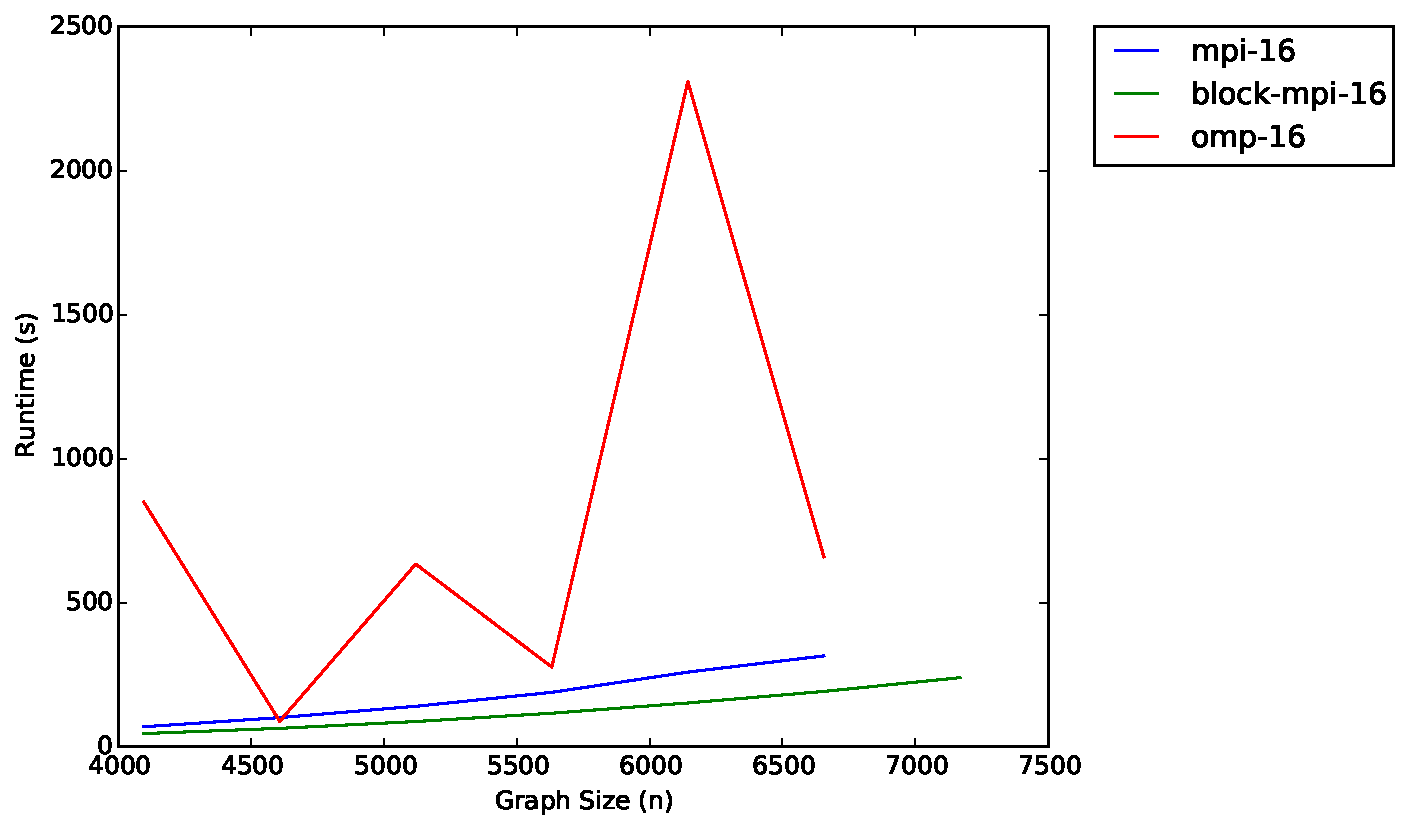
\includegraphics[width=\textwidth]{comparison_large.pdf}
		\caption{Large problem sizes}
	\end{subfigure}
	\caption{Speed of the three implementations as the problem size increases; block-mpi is our tuned MPI implementation}
	\label{fig:size-comparison}
\end{figure*}


\subsection{Strong Scaling Study}

Next, we measured how much paralellism our code is able to exploit by setting up a strong scaling study.
We chose a fixed problem size of n=3072 because this seemed to be a large enough problem for parallelism to make a difference, without being one of the sizes that causes problems for OpenMP.
Figure \ref{fig:strong-scaling-time} shows how the completion time of the problem decreases as we add more processors, while Figure \ref{fig:strong-scaling-speedup} shows the speedup of each program over the serial version of that program.

With an ideal parallel implementation, speedup would increase linearly as the number of processors increases.
However, all of these implementations show speedups that level out as the number of processors increases due to synchronization overheads.
For all implementations, the largest speedup (and largest change in running time) occurs with the change from 1 to 4 processors.
Additional parallelism after 4 is less effective, especially for our tuned MPI implementation.
This is probably the result of the fact that our tuned MPI implementation has a more efficient kernel and thus has less serial work to do per iteration (as evidenced by its far lower runtime for the single-threaded case), so there is less work to be split among processors and less room for speedup compared to the single-threaded version.
In fact, with 16 processors our tuned MPI implementation actually runs slightly slower than with 9 processors, which reflects the additional communication overhead of more processors (and more communication groups) dominating the speedup gained by splitting the matrix into more parallel blocks.
On the other hand, our non-tuned MPI implementation has a speedup that is closer to linear than the OpenMP implementation, which confirms our prediction that splitting the matrix by both rows and columns would decrease communication overhead compared to the column-only decomposition used in the OpenMP code.

\begin{figure*}[ht]
	\centering
	\begin{subfigure}[b]{.45\textwidth}
		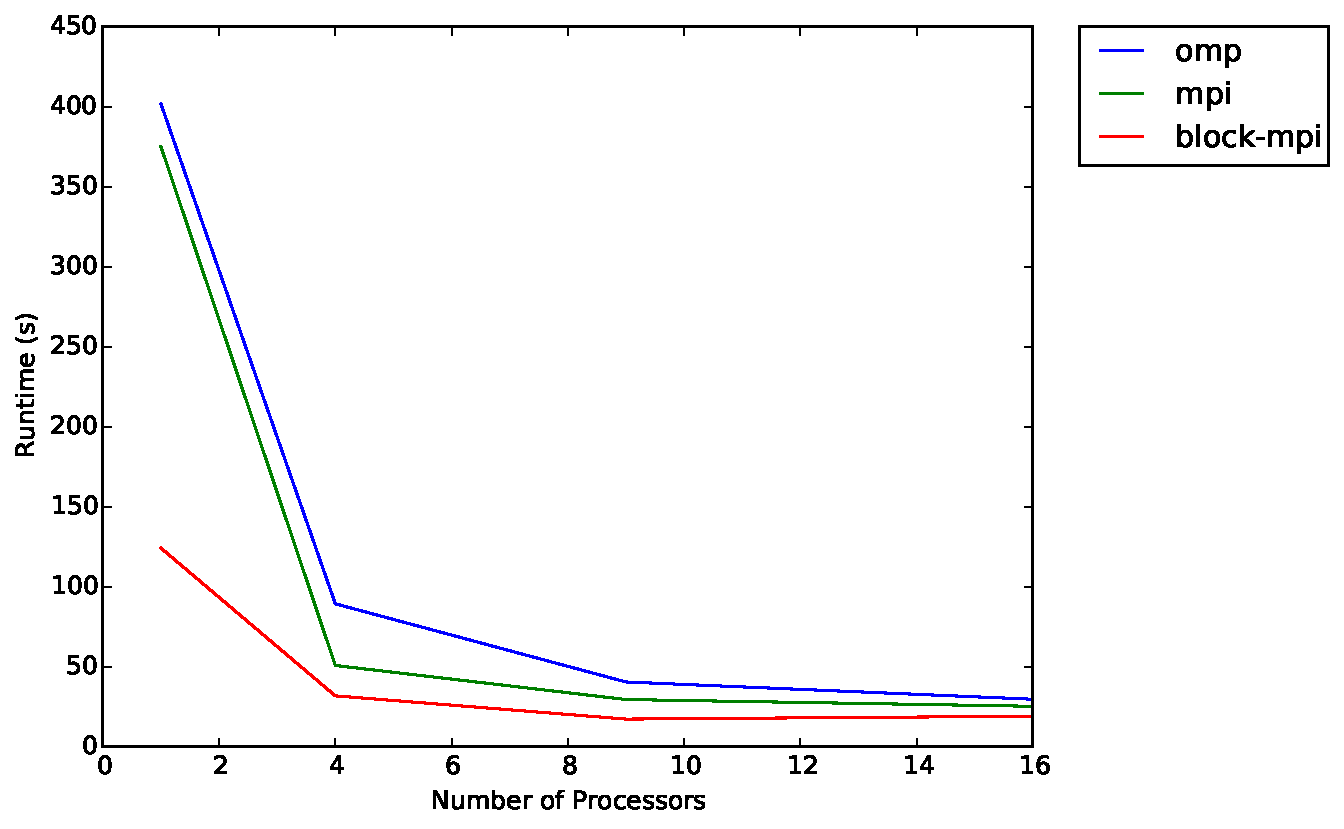
\includegraphics[width=\textwidth]{strong-scaling-time.pdf}
		\caption{Scaling measured by total running time}
		\label{fig:strong-scaling-time}
	\end{subfigure}
	\begin{subfigure}[b]{.45\textwidth}
		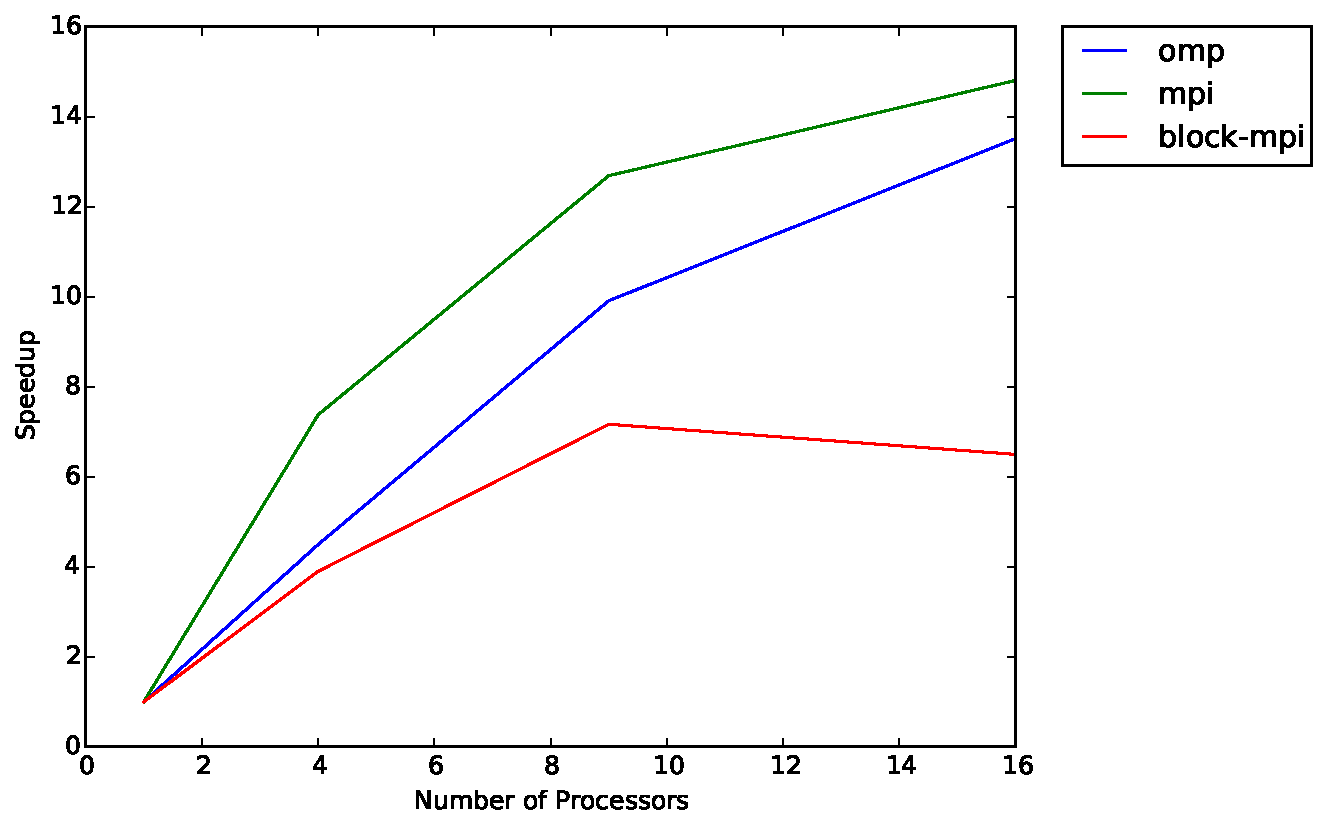
\includegraphics[width=\textwidth]{strong-scaling-speedup.pdf}
		\caption{Scaling measured by speedup}
		\label{fig:strong-scaling-speedup}
	\end{subfigure}
	\caption{Strong scaling study results for the three algorithms with n=3072}
	\label{fig:strong-scaling}
\end{figure*}

\subsection{Weak Scaling Study}

We also measured our code's scaling efficiency by setting up a weak scaling study.
We chose a per-processor problem size of n=1024, so that the larger numbers of processors would have large enough problem sizes to show a benefit from parallelism (i.e. 3072, 4096).
Figure \ref{fig:weak-scaling-time} shows the completion times of each implementation as both the problem size and the number of processors increases, and Figure \ref{fig:weak-scaling-percent} shows the scaled speedup, or efficiency, of each implementation as a percentage of the ideal linear scaling. 
Note that the problem size we chose meant that the OpenMP code encountered its severe failure case of n=4096, taking 695 seconds to complete with 16 threads.
In order to make Figure \ref{fig:weak-scaling-time} readable, we truncated the y-axis at 250, and do not show the data point for OpenMP with 16 processors.

\begin{figure*}[ht]
	\centering
	\begin{subfigure}[b]{.45\textwidth}
		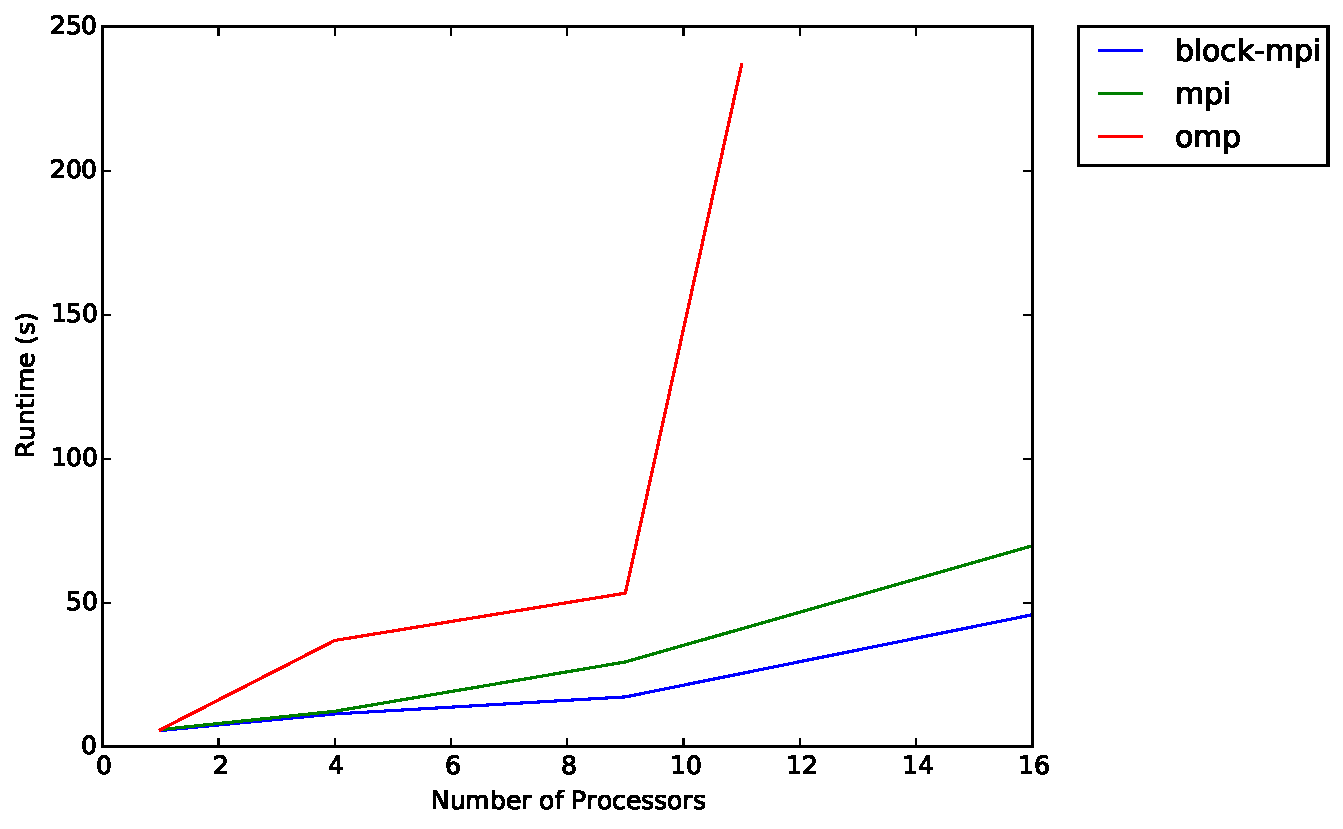
\includegraphics[width=\textwidth]{weak-scaling-time.pdf}
		\caption{Scaling measured by total running time}
		\label{fig:weak-scaling-time}
	\end{subfigure}
	\begin{subfigure}[b]{.45\textwidth}
		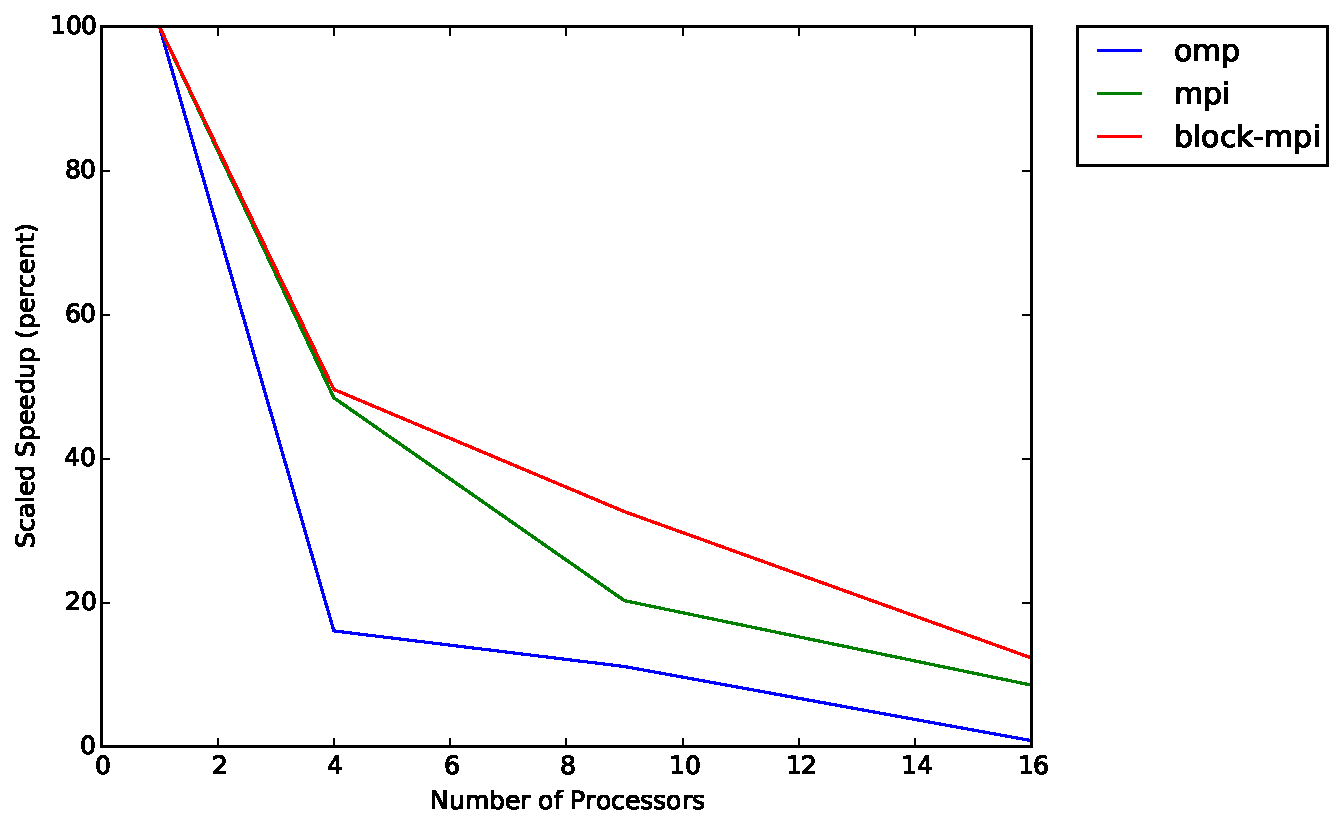
\includegraphics[width=\textwidth]{weak-scaling-percent.pdf}
		\caption{Scaling measured by weak scaling efficiency}
		\label{fig:weak-scaling-percent}
	\end{subfigure}
	\caption{Weak scaling study results for the three algorithms with per-processor block dimensions of 1024 (n=1024$\sqrt{p}$)}
	\label{fig:weak-scaling}
\end{figure*}

With an ideal parallel implementation, the completion time of the problems would remain constant as the problem size increases (since the amount of work per processor remains constant).
This would correspond to 100\% efficiency in the speedup graph.
However, all of these algorithms show gradually increasing runtime as the problem size increases, due to synchronization and communication overheads.
The OpenMP code shows the worst scaling, jumping dramatically in runtime as soon as more than one processor is added, due to the high synchronization and communication costs incurred by its rather naive algorithm.
Our MPI code scales better, and the primary benefit seems to be from the better communication pattern, as the initial and tuned MPI implementations are much closer to each other than to the OpenMP implementation.
Fortunately, our tuned MPI code does have some advantage, maintaining better efficiency at large numbers of processors.
This is likely due to its cache-friendliness, since larger numbers of processors mean more memory traffic (and hence longer delays) at the same rate of cache misses per processor.

\section{Future Work}
There is more that we could do with our MPI implementation if we had more time. 
For example, we could add additional blocking logic to accommodate non-square numbers of processors; the solution we had planned on implementing would be to round up the number of large blocks to the next largest square number, and assign multiple blocks to each processor to make up the difference.
This would entail putting a single processor in more than one row or column, however, so we would need to develop a strategy to reduce the communication stress on multi-block processors in this case.
We would also like to test the performance of the second-level blocking at different sizes for the small blocks, to ensure they are properly tuned to the cache size of the Xeon processors.

\end{document}
